\section{Descriptives of the number of responses}

\begin{longtable}[c]{@{}lrrrrrrrrrr@{}}
\caption{Flashcard condition}
\endfirsthead
\endhead
\toprule\addlinespace
& sample & min & max & mean & variance & skew & kurtosis & normal-t &
normal-p & $\alpha$
\\\addlinespace
\midrule\endhead
\textbf{abs} & 12 & 298 & 915 & 408.17 & 28248.33 & 2.53 & 5.26 & 26.675
& 0.0000 & 0.8557
\\\addlinespace
\textbf{rel} & 12 & 6 & 19 & 8.87 & 13.35 & 2.53 & 5.26 & 26.675 &
0.0000 & 0.8557
\\\addlinespace
\bottomrule
\end{longtable}

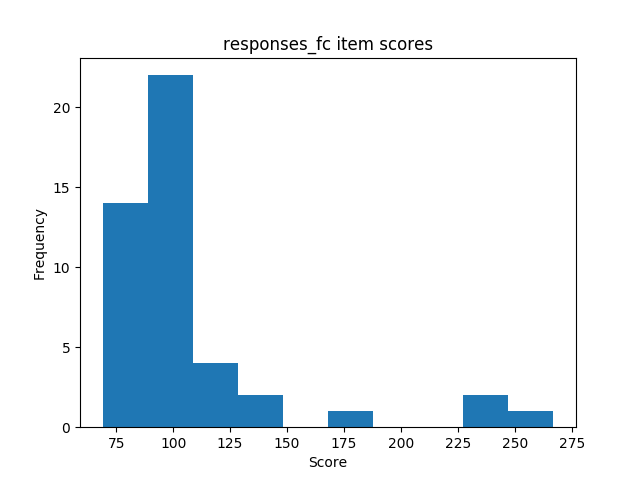
\includegraphics{responses_fc_diff.png}
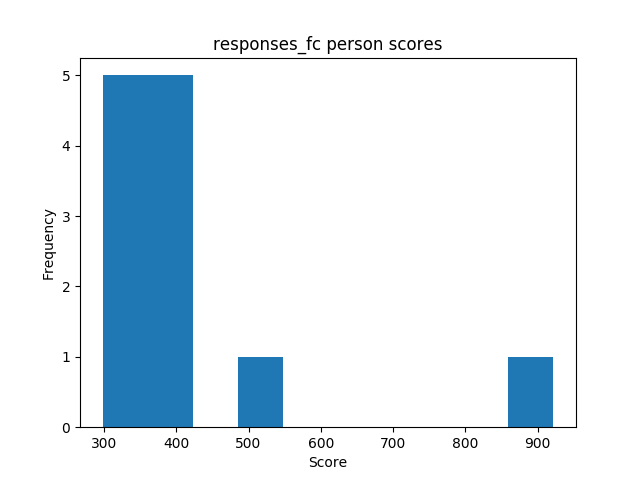
\includegraphics{responses_fc_abil.png}

\begin{longtable}[c]{@{}lrrrrrrrrrr@{}}
\caption{Flashmap condition}
\endfirsthead
\endhead
\toprule\addlinespace
& sample & min & max & mean & variance & skew & kurtosis & normal-t &
normal-p & $\alpha$
\\\addlinespace
\midrule\endhead
\textbf{abs} & 11 & 278 & 471 & 374.36 & 4875.05 & 0.13 & -1.28 & 1.516
& 0.4686 & 0.7098
\\\addlinespace
\textbf{rel} & 11 & 5 & 9 & 7.49 & 1.95 & 0.13 & -1.28 & 1.516 & 0.4686
& 0.7098
\\\addlinespace
\bottomrule
\end{longtable}

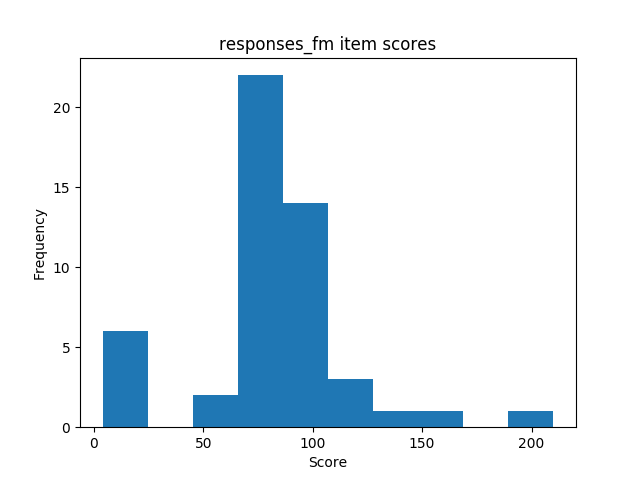
\includegraphics{responses_fm_diff.png}
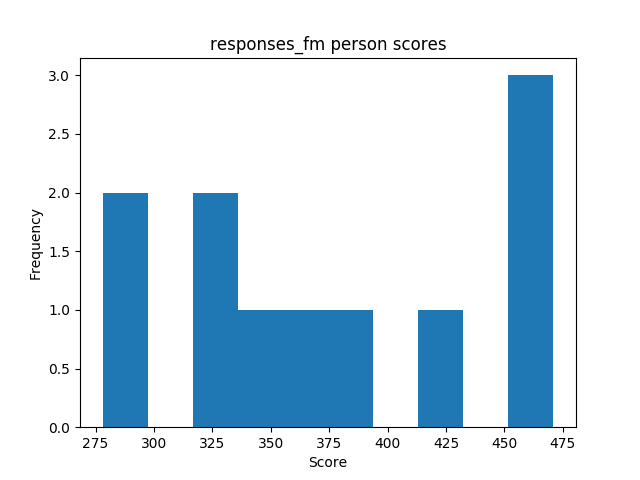
\includegraphics{responses_fm_abil.png}

\begin{longtable}[c]{@{}lrrrrrrrrrr@{}}
\caption{Combined conditions}
\endfirsthead
\endhead
\toprule\addlinespace
& sample & min & max & mean & variance & skew & kurtosis & normal-t &
normal-p & $\alpha$
\\\addlinespace
\midrule\endhead
\textbf{abs} & 23 & 328 & 1230 & 474.74 & 34192.57 & 3.12 & 10.33 &
41.081 & 0.0000 & 0.8731
\\\addlinespace
\textbf{rel} & 23 & 6 & 24 & 9.31 & 13.15 & 3.12 & 10.33 & 41.081 &
0.0000 & 0.8731
\\\addlinespace
\bottomrule
\end{longtable}

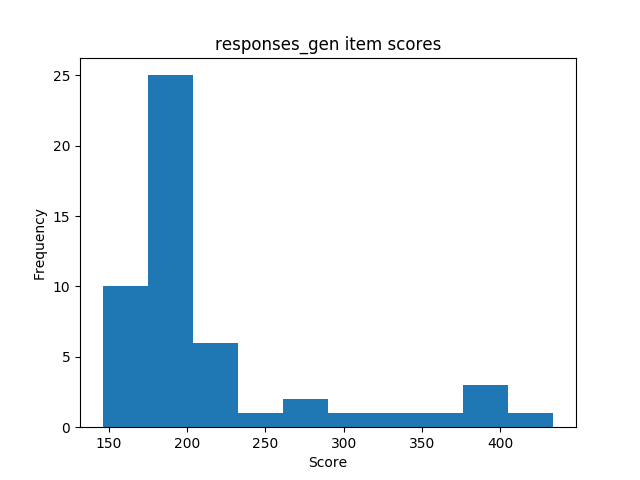
\includegraphics{responses_gen_diff.png}
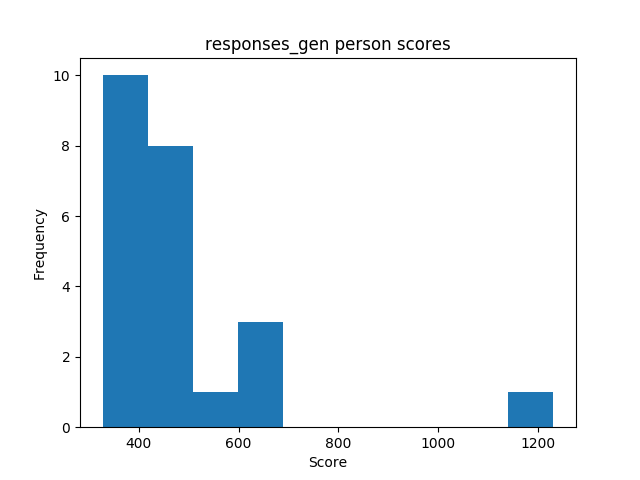
\includegraphics{responses_gen_abil.png}

\section{Descriptives of percentage of responses marked as correct}

\begin{longtable}[c]{@{}lrrrrrrrrrr@{}}
\caption{Flashcard condition}
\endfirsthead
\endhead
\toprule\addlinespace
& sample & min & max & mean & variance & skew & kurtosis & normal-t &
normal-p & $\alpha$
\\\addlinespace
\midrule\endhead
\textbf{abs} & 12 & 35 & 43 & 40.42 & 4.04 & -1.15 & 1.74 & 8.672 &
0.0131 & 0.9106
\\\addlinespace
\textbf{rel} & 12 & 0 & 0 & 0.88 & 0.00 & -1.15 & 1.74 & 8.672 & 0.0131
& 0.9106
\\\addlinespace
\bottomrule
\end{longtable}

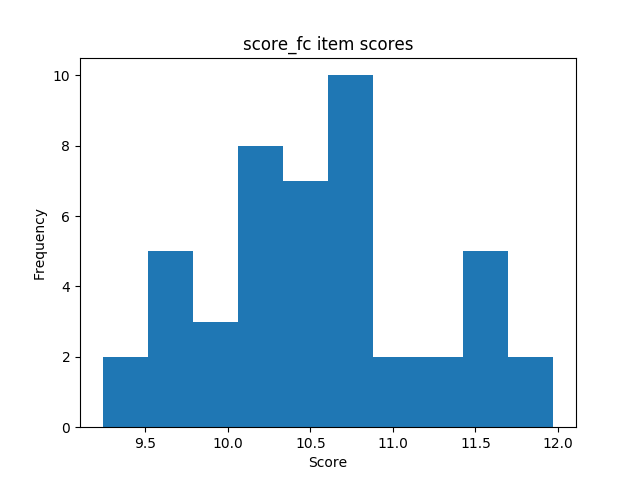
\includegraphics{score_fc_diff.png} 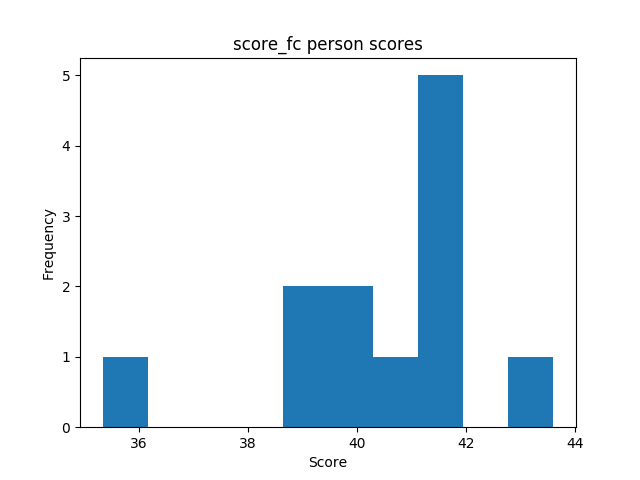
\includegraphics{score_fc_abil.png}

\begin{longtable}[c]{@{}lrrrrrrrrrr@{}}
\caption{Flashmap condition}
\endfirsthead
\endhead
\toprule\addlinespace
& sample & min & max & mean & variance & skew & kurtosis & normal-t &
normal-p & $\alpha$
\\\addlinespace
\midrule\endhead
\textbf{abs} & 11 & 43 & 51 & 47.11 & 6.19 & 0.31 & -1.17 & 1.231 &
0.5404 & 0.9511
\\\addlinespace
\textbf{rel} & 11 & 0 & 1 & 0.92 & 0.00 & 0.31 & -1.17 & 1.231 & 0.5404
& 0.9511
\\\addlinespace
\bottomrule
\end{longtable}

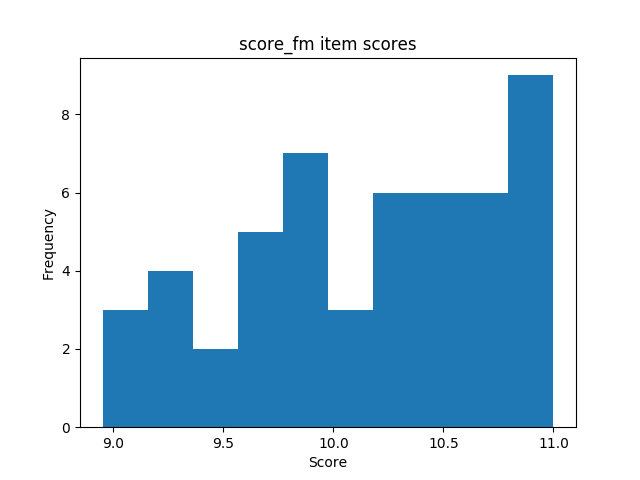
\includegraphics{score_fm_diff.png} 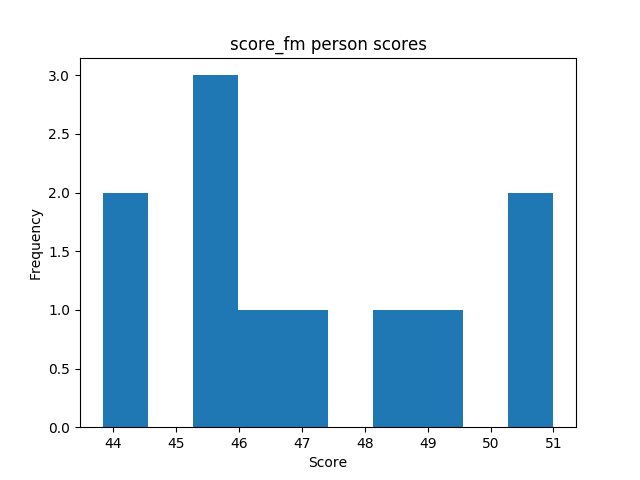
\includegraphics{score_fm_abil.png}

\begin{longtable}[c]{@{}lrrrrrrrrrr@{}}
\caption{Combined conditions}
\endfirsthead
\endhead
\toprule\addlinespace
& sample & min & max & mean & variance & skew & kurtosis & normal-t &
normal-p & $\alpha$
\\\addlinespace
\midrule\endhead
\textbf{abs} & 23 & 40 & 51 & 45.97 & 6.47 & 0.06 & 0.22 & 0.711 &
0.7008 & 0.9459
\\\addlinespace
\textbf{rel} & 23 & 0 & 1 & 0.90 & 0.00 & 0.06 & 0.22 & 0.711 & 0.7008 &
0.9459
\\\addlinespace
\bottomrule
\end{longtable}

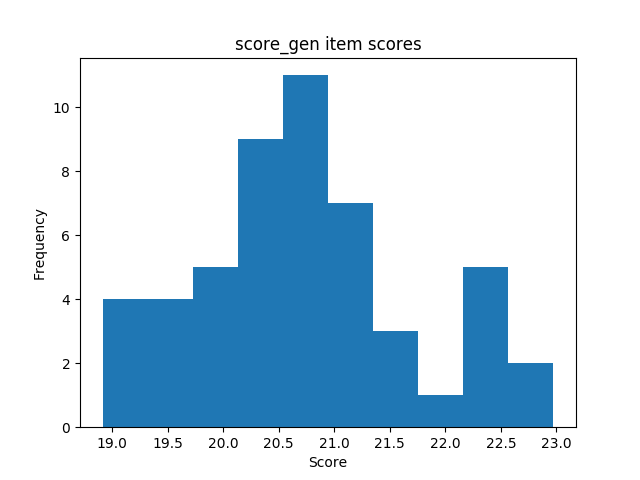
\includegraphics{score_gen_diff.png}
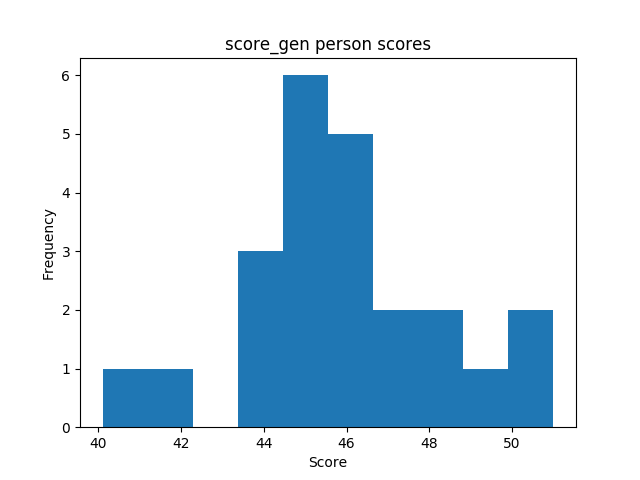
\includegraphics{score_gen_abil.png}

\subsubsection{Descriptives of the amount of time spent on the application}

\begin{longtable}[c]{@{}lrrrrrrrrrr@{}}
\caption{Flashcard condition}
\endfirsthead
\endhead
\toprule\addlinespace
& sample & min & max & mean & variance & skew & kurtosis & normal-t &
normal-p & $\alpha$
\\\addlinespace
\midrule\endhead
\textbf{abs} & 12 & 1544 & 12345 & 8173.94 & 10611999.29 & -0.77 & -0.33
& 2.156 & 0.3402 & 0.8776
\\\addlinespace
\textbf{rel} & 12 & 33 & 268 & 177.69 & 5015.12 & -0.77 & -0.33 & 2.156
& 0.3402 & 0.8776
\\\addlinespace
\bottomrule
\end{longtable}

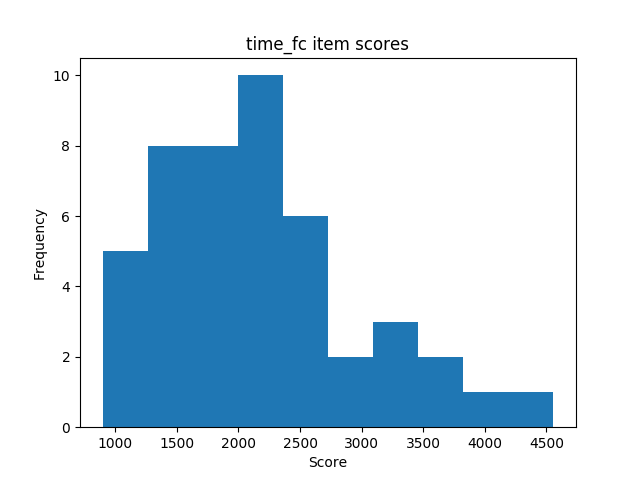
\includegraphics{time_fc_diff.png} 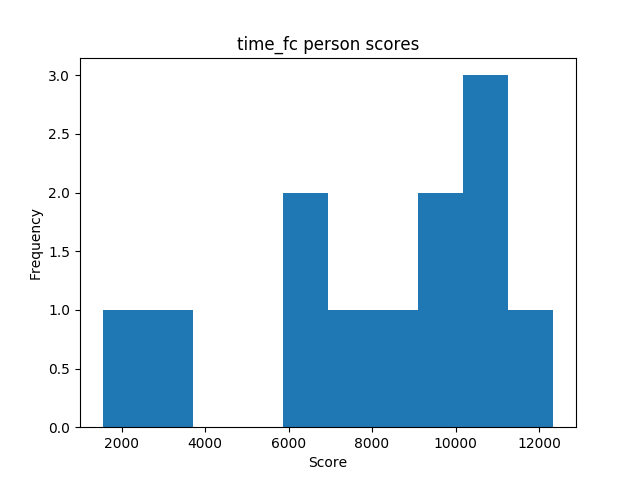
\includegraphics{time_fc_abil.png}

\begin{longtable}[c]{@{}lrrrrrrrrrr@{}}
\caption{Flashmap condition}
\endfirsthead
\endhead
\toprule\addlinespace
& sample & min & max & mean & variance & skew & kurtosis & normal-t &
normal-p & $\alpha$
\\\addlinespace
\midrule\endhead
\textbf{abs} & 11 & 1707 & 12233 & 7221.30 & 8917086.17 & 0.05 & -0.44 &
0.092 & 0.9551 & 0.8268
\\\addlinespace
\textbf{rel} & 11 & 34 & 244 & 144.43 & 3566.83 & 0.05 & -0.44 & 0.092 &
0.9551 & 0.8268
\\\addlinespace
\bottomrule
\end{longtable}

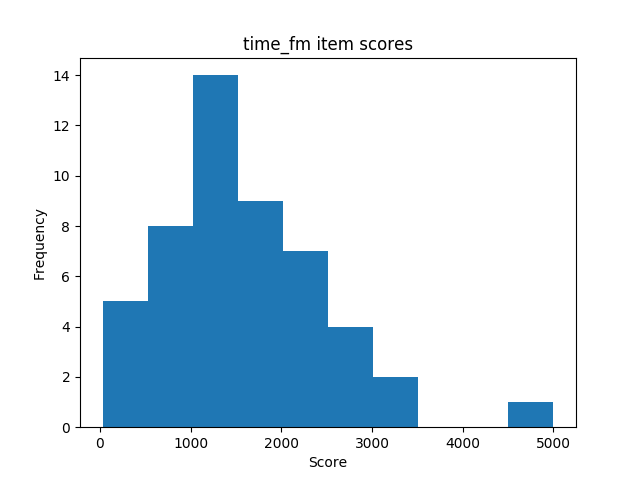
\includegraphics{time_fm_diff.png} 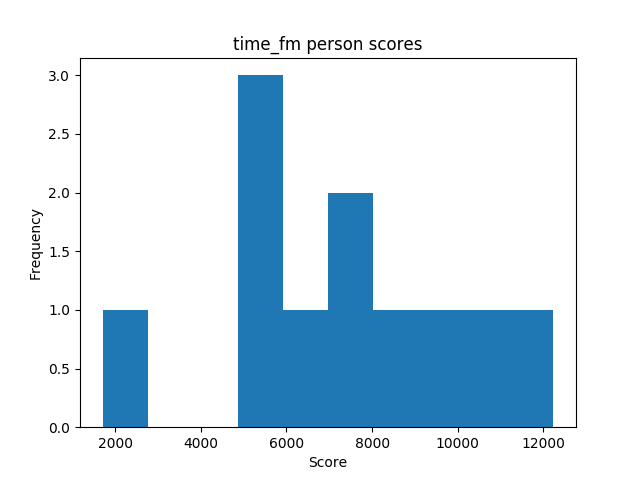
\includegraphics{time_fm_abil.png}

\begin{longtable}[c]{@{}lrrrrrrrrrr@{}}
\caption{Combined conditions}
\endfirsthead
\endhead
\toprule\addlinespace
& sample & min & max & mean & variance & skew & kurtosis & normal-t &
normal-p & $\alpha$
\\\addlinespace
\midrule\endhead
\textbf{abs} & 23 & 1426 & 16484 & 9283.95 & 14203173.83 & -0.31 & -0.29
& 0.544 & 0.7617 & 0.8591
\\\addlinespace
\textbf{rel} & 23 & 27 & 323 & 182.04 & 5460.66 & -0.31 & -0.29 & 0.544
& 0.7617 & 0.8591
\\\addlinespace
\bottomrule
\end{longtable}

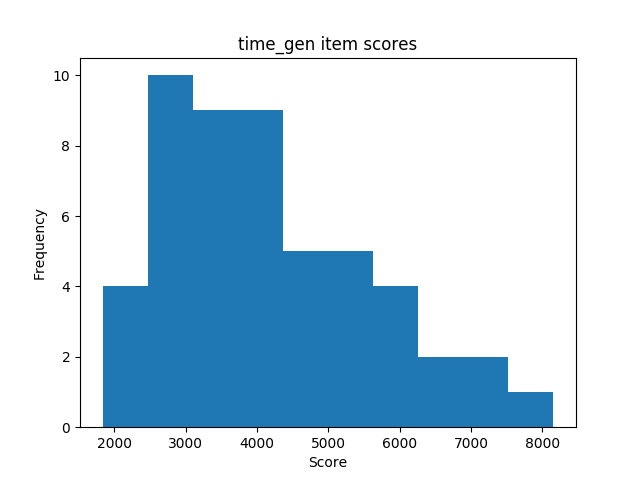
\includegraphics{time_gen_diff.png} 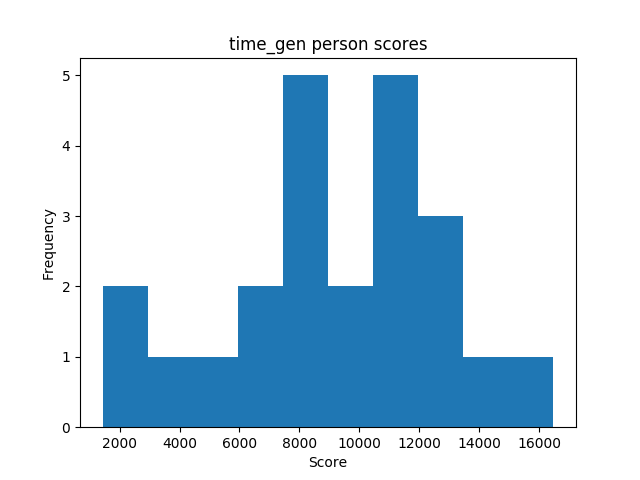
\includegraphics{time_gen_abil.png}

\section{Comparisons of the number of responses}

\begin{longtable}[c]{@{}lrrrr@{}}
\toprule\addlinespace
& \textbf{Mann-Whitney-U k} & \textbf{Mann-Whitney-U p} &
\textbf{Welch's t-test k} & \textbf{Welch's t-test p}
\\\addlinespace
\midrule\endhead
\textbf{abs} & 0.619 & 0.5426 & 0.639 & 0.5324
\\\addlinespace
\textbf{rel} & 1.180 & 0.2513 & 1.220 & 0.2420
\\\addlinespace
\bottomrule
\end{longtable}

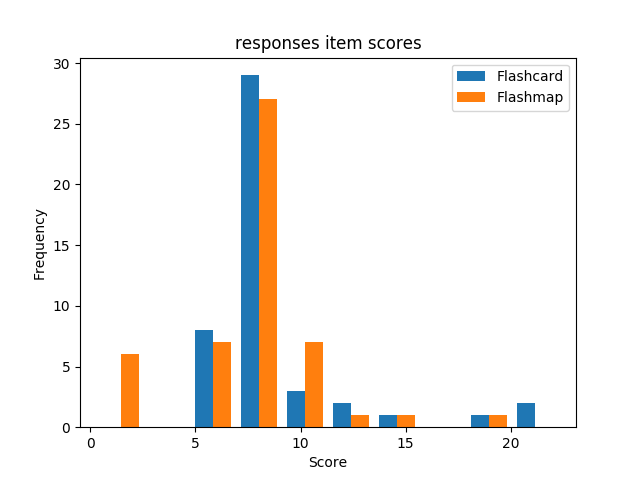
\includegraphics{responses_diff.png}
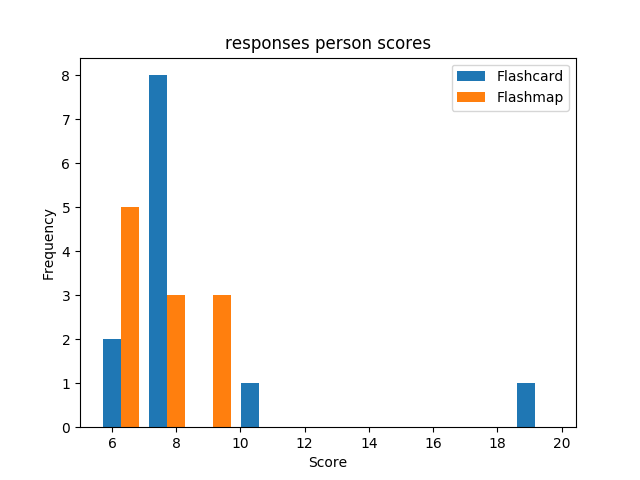
\includegraphics{responses_abil.png}

\section{Comparisons of the percentage of responses marked as correct}

\begin{longtable}[c]{@{}lrrrr@{}}
\toprule\addlinespace
& \textbf{Mann-Whitney-U k} & \textbf{Mann-Whitney-U p} &
\textbf{Welch's t-test k} & \textbf{Welch's t-test p}
\\\addlinespace
\midrule\endhead
\textbf{abs} & -16.597 & 0.0000 & -15.857 & 0.0000
\\\addlinespace
\textbf{rel} & -16.421 & 0.0000 & -15.689 & 0.0000
\\\addlinespace
\bottomrule
\end{longtable}

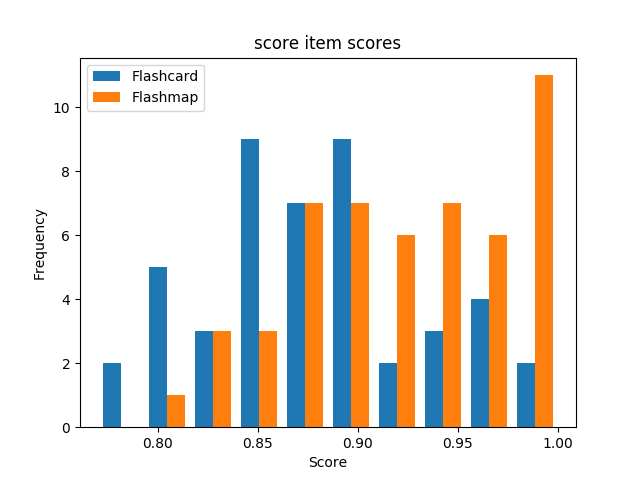
\includegraphics{score_diff.png} 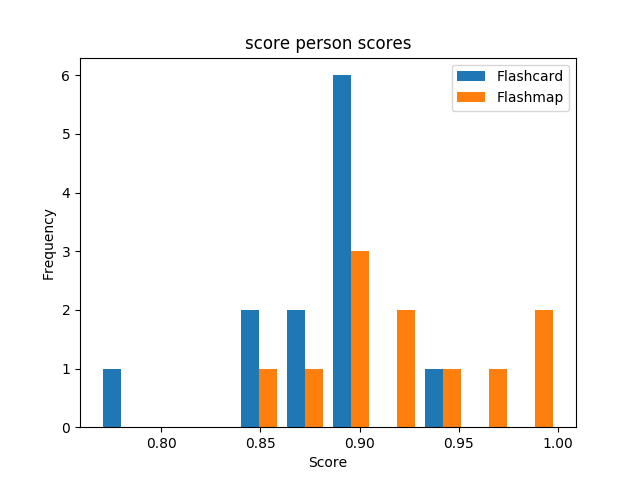
\includegraphics{score_abil.png}

\section{Comparisons of the amount of time spent on the application}

\begin{longtable}[c]{@{}lrrrr@{}}
\toprule\addlinespace
& \textbf{Mann-Whitney-U k} & \textbf{Mann-Whitney-U p} &
\textbf{Welch's t-test k} & \textbf{Welch's t-test p}
\\\addlinespace
\midrule\endhead
\textbf{abs} & 7.924 & 0.0000 & 8.292 & 0.0000
\\\addlinespace
\textbf{rel} & 7.954 & 0.0000 & 8.324 & 0.0000
\\\addlinespace
\bottomrule
\end{longtable}

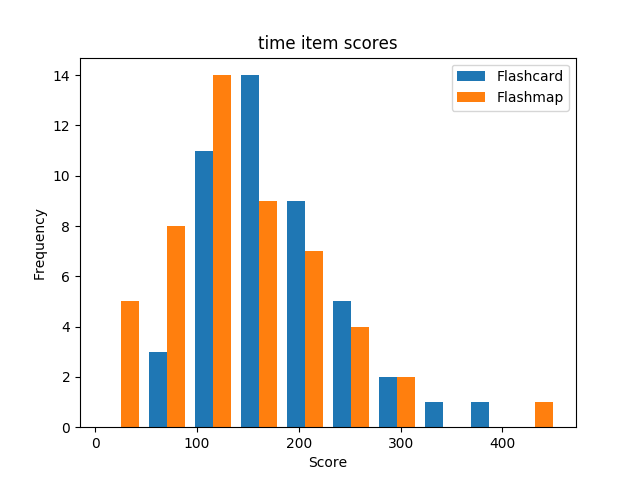
\includegraphics{time_diff.png} 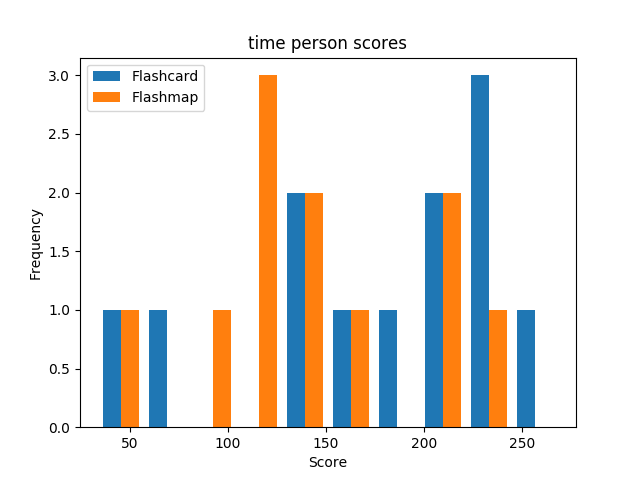
\includegraphics{time_abil.png}
